\documentclass{article}
\usepackage{geometry}
\usepackage{algorithmic}
%\usepackage{fancyhdr}
\usepackage{amsmath,amsthm,amssymb}
\usepackage{graphicx}
\usepackage{hyperref}
\usepackage{enumerate}
\usepackage{caption}

\newcommand{\argmax}{\operatornamewithlimits{argmax}}

\title{Parallelizing Stochastic Gradient Descent}
\author{Kirstin Early \qquad Nicole Rafidi}
%\date{\today}

\begin{document}
\maketitle

\section{Introduction}
Gradient descent (also called coordinate descent) is a popular numerical technique for optimizing an expression that has no closed-form solution. This method can find a local minimum of a differentiable function by iteratively moving an initial guess of the minimum value in the opposite direction of the gradient at that point, either for a pre-specified number or iterations or until the update does not change the estimated value significantly. The latter case is typically named convergence. In this project, we discuss convergence properties after running for a pre-specified number of iterations in terms of the error rate of the resulting estimation. We say that an algorithm has good convergence properties if it quickly reaches a near-optimal error rate. In the multivariate case, it is possible to update each coordinate individually in this manner. When data are numerous, stochastic gradient descent can improve efficiency by performing the update using a random subset of training examples or on a subset of features at each step.

In this project, we examine the performance improvement gained by parallelizing various sections of the stochastic gradient descent algorithm with OpenMP. We optimize the objective function for logistic regression with $L_2$ regularization:
\begin{equation}
\underset{w}{\min}-\frac{1}{1 + \exp(-y \cdot w^T x)} + \frac{\lambda}{2}||w||^2_2,
\end{equation}
where $x \in \mathbb{R}^F$ is a vector of sample features, $y \in \lbrace -1, 1 \rbrace$ is the sample label, and $w \in \mathbb{R}^F$ is a vector of feature weights. The first term in the optimization objective is the negative conditional likelihood of a sample's label given its features, $p(y|x)$; the second term is a regularization penalty on $w$. Sparse solutions (those solutions with few nonzero weights in $w$) are particularly desirable when the number of features exceeds the number of samples.

The optimum value for this objective function has no closed-form solution, and so we use gradient descent to find the minimum value. Letting $x \in \mathbb{R}^{N \times F}$ be the matrix of $N$ samples with $F$ features each, the update equation for a particular feature weight $w_f$ is
\begin{equation}
w_f = w_f + \eta \left( \sum_{i = 1}^{N}(y_i - g(w_f, x_{i, f})) + \lambda w_f \right)
\end{equation}
\begin{equation}
g(w_f, x_{i,f}) = \frac{-w_fx_{i,f} e^{-w_fx_{i,f}}}{1 + e^{-w_fx_{i,f}}}
\end{equation}

Here, $\eta$ is a step size parameter that indicates the size of the update on each iteration.

After learning the weight vector $w$, we can predict the label of a new vector $x$ by $\hat{y} = sgn(w^Tx)$. This prediction captures the relationship between $w$ and the conditional likelihood $p(y|x)$: when $p(y = 1|x) > \frac{1}{2}$, $w^Tx$ is positive, and vice versa.

\section{Related Work}
Several recent studies have also looked at parallelizing stochastic gradient descent. The Shotgun project parallelized $L_1$-regularized coordinate descent over features, proved near-linear speedup for their parallel algorithm, and empirically supported this theoretical result on several large datasets \cite{shotgun2011}. The Hogwild! project also theoretically proves near-linear speedup for sample-parallelized stochastic gradient descent under sparsity, even when the updates are made non-atomically: a lock-free approach does not often result in memory overwrites when the data are sparse because few parallel computations try to modify the same variable concurrently \cite{hogwild2011}. However, Hogwild! does assume that each the additive update to a component of the weight vector is an atomic operation; our implementation respects this atomicity when updating a weight element across samples, but not across features. This assumption is not as strong as Hogwild's since, by definition, Hogwild! also enforces atomic addition across features since Hogwild! does not parallelize over features.

\section{Algorithms and Optimizations}
\subsection{Stochastic Gradient Descent}
In this project we implemented stochastic gradient descent for $L_2$ penalized logistic regression. The mathematical basis of this algorithm was explained in the Inroduction. Here we give pseudocode of the algorithms involved.
\\
\\
\begin{tabular} {l}
\hline
\hline
Algorithm 1 \\
\hline
\end{tabular}
\begin{algorithmic}
\STATE $w \leftarrow 0$ 
\WHILE{!converged} 
\FOR{$i = 0$ \TO $F-1$} 
\FOR{$j = 0$ \TO $N-1$} 
\STATE $w[i] \leftarrow w[i] + \eta(y[j] - g(w[i], x[i, j]))$ 
\ENDFOR 
\STATE $w[i] \leftarrow w[i] + \eta\lambda w[i]$ 
\ENDFOR 
\ENDWHILE 
\end{algorithmic}
Algorithm 1 is the generic gradient descent. If the number of features is large, it can be very time consuming to update all features on each iteration of the algorithm, especially if it is likely that not all features are informative.  Thus, in stochastic gradient descent, a feature (or a set of features) is randomly chosen and its weight updated on each iteration using all or a subset of the training samples. This is shown in Algorithm 2.
\\
\\
\begin{tabular}{l}
\hline
\hline
Algorithm 2 \\
\hline
\end{tabular}
\begin{algorithmic}
\STATE $w \leftarrow 0$
\FOR{$t = 0$ \TO $num_iterations$}
\FOR{$i = 0$ \TO $batch_F$}
\STATE choose $f$ randomly from $F$
\FOR{$j = 0$ \TO $batch_N$}
\STATE choose $n$ randomly from $N$
\STATE $w[f] \leftarrow w[f] + \eta(y[n] - g(w[f], x[f, n]))$
\ENDFOR
\STATE $w[f] \leftarrow w[f] + \eta\lambda w[f]$
\ENDFOR
\ENDFOR
\end{algorithmic}
\subsection{Parallelized Versions}
There are several ways in which Algorithm 2 can be parallelized. In this project we explore two ways of parallelizing: batch updates, and a parallelization of those batch updates.  In each iteration, rather than updating the weight corresponding to one feature, which will require a large number of iterations to converge, we can update a subset of the weights (a batch).  If the probability that the same weight will appear more than once in a batch is low, then all the weights in the batch can be updated in parallel safely. We can also vary how many samples are used in each update.  Using too few will greatly increase the number of iterations needed to converge, but using all samples may not be necessary, either.  Updating a weight is simply adding an independent value to it.  Thus, we can parallelize the weight update across samples with minimal conflict in the result.

There are four levels of parallelization that we explored in this project:
\begin{enumerate}
\item
No parallelization
\item
Parallelization across samples; updating a weight with the samples in a batch in parallel
\item
Parallelization across features; updating all the weights in a batch in parallel
\item
Parallelization of both loops
\end{enumerate}
\subsection{Experiments}
Our goal was to see how the benefits gained by each level of parallelization change as the batch sizes are increased.  To that end, we ran Algorithm 2 at each level of parallelization, for varying batch sizes and compared the performance on a validation set as well as the runtime. The number of iterations and the step size were fixed throughout, and the regularization constant $\lambda$ was chosen with cross-validation of the training set for each feature and sample batch size pair. The only operation that was made atomic was the update over samples within an update of a particular weight (e.g. the innermost loop of Algorithm 2).
\subsubsection{Data Sets}
We used the ijcnn1 data set from among those used by \cite{shotgun2011}. The data consisted of 22 features and 45000  samples, which we divided in half for a training and a validation set.
\subsubsection{Code Structure}
Our main file, which runs the experiments, is runexp.c.  It calls functions from data_proc.c and scd.c. All files and their corresponding header files are included at the end of the report.

\section{Results}
\subsection{Runtime Analysis}
As Figures~\ref{fig:time_samp} and \ref{fig:time_feat} show, increasing the level of parallelization in stochastic gradient descent can improve the runtime up to a certain extent. With no parallelization, the runtime increases roughly linearly as batch sizes increase, in both dimensions. However, once updates across samples or features are made parallel, the runtime reaches a plateau and remains constant. Parallelizing over features reaches this plateau sooner than parallelizing over samples alone; making both feature and sample batch updates in parallel results in the most speedup.  There is of course an increased startup cost to parlallelization which can be attributed to scheduling. However, as the numbers of features and samples increase, it pays off to parallelize.
\begin{figure}
\centering
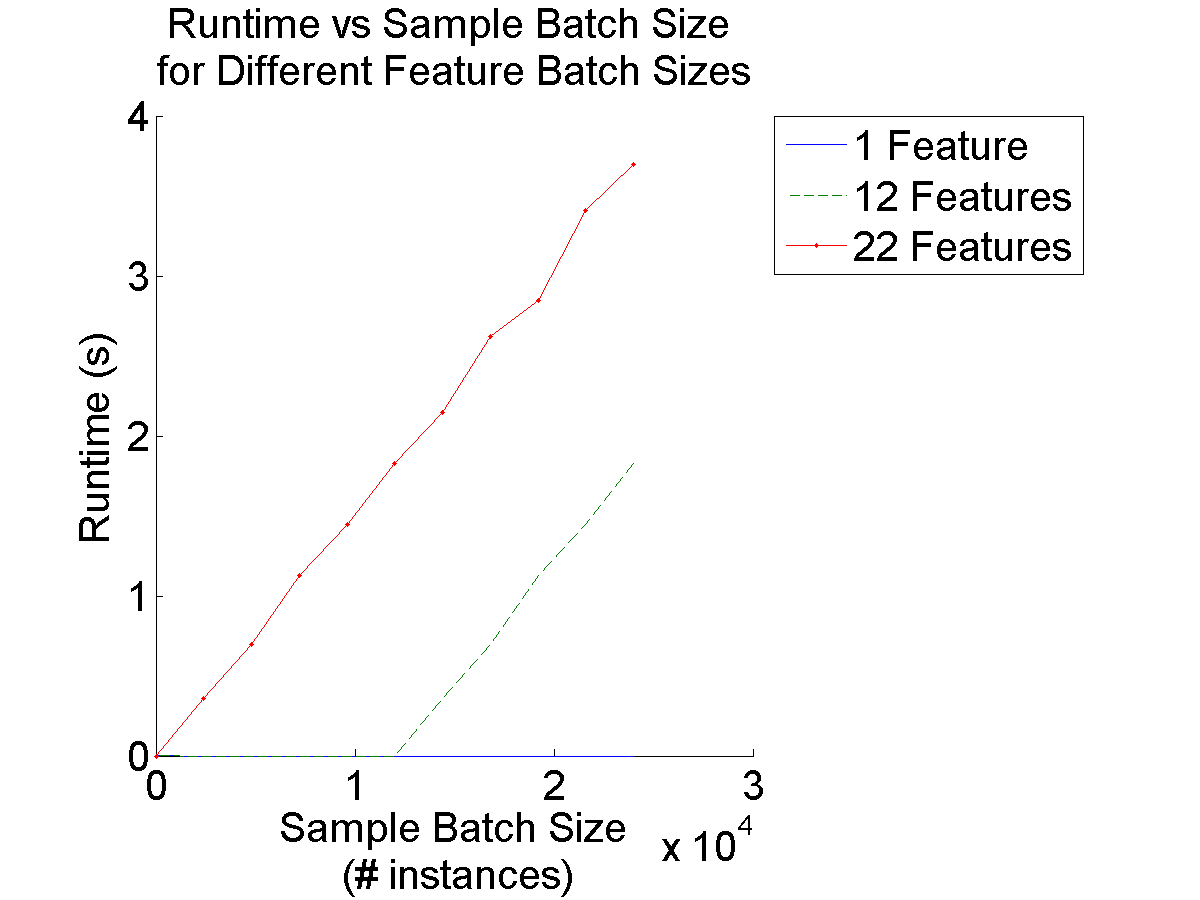
\includegraphics[width = .4\linewidth]{samptimeplot5}
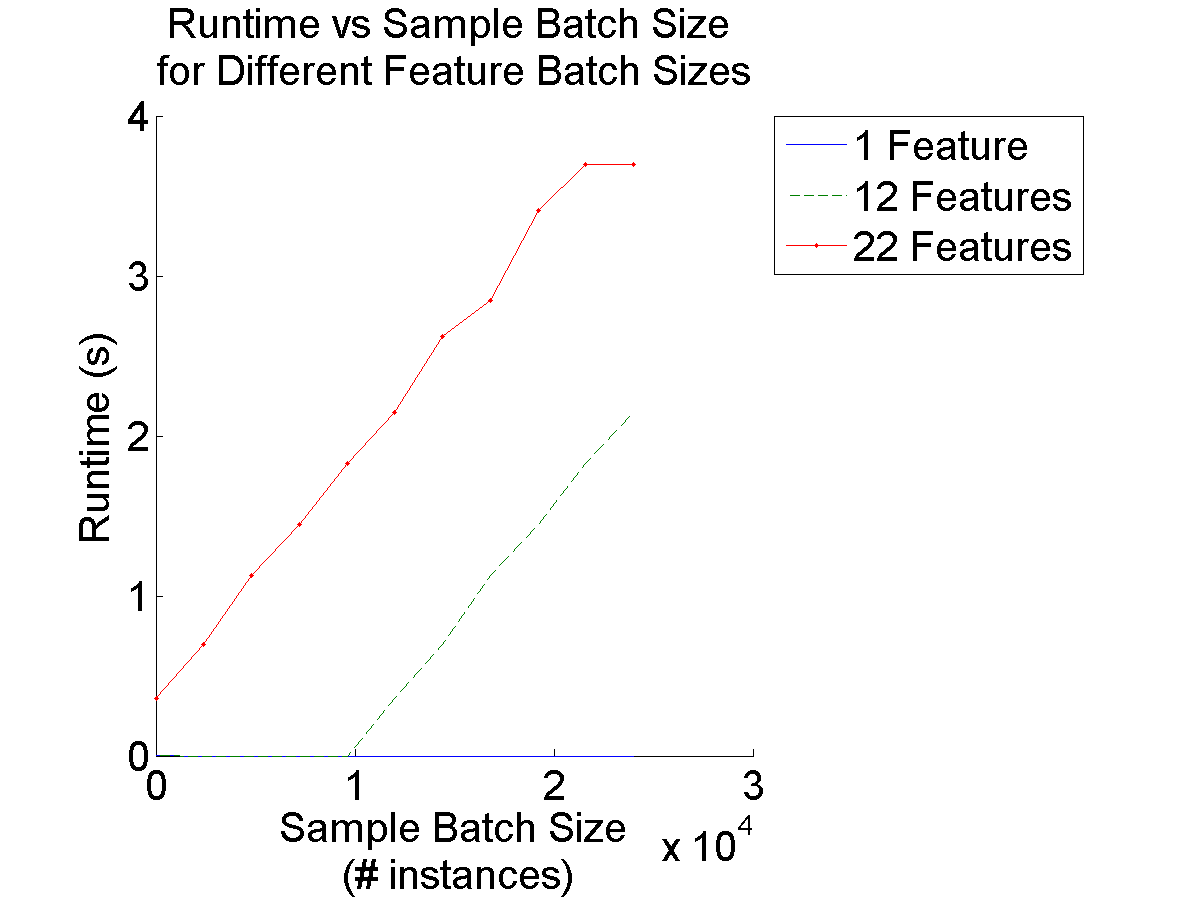
\includegraphics[width = .4\linewidth]{samptimeplot7}
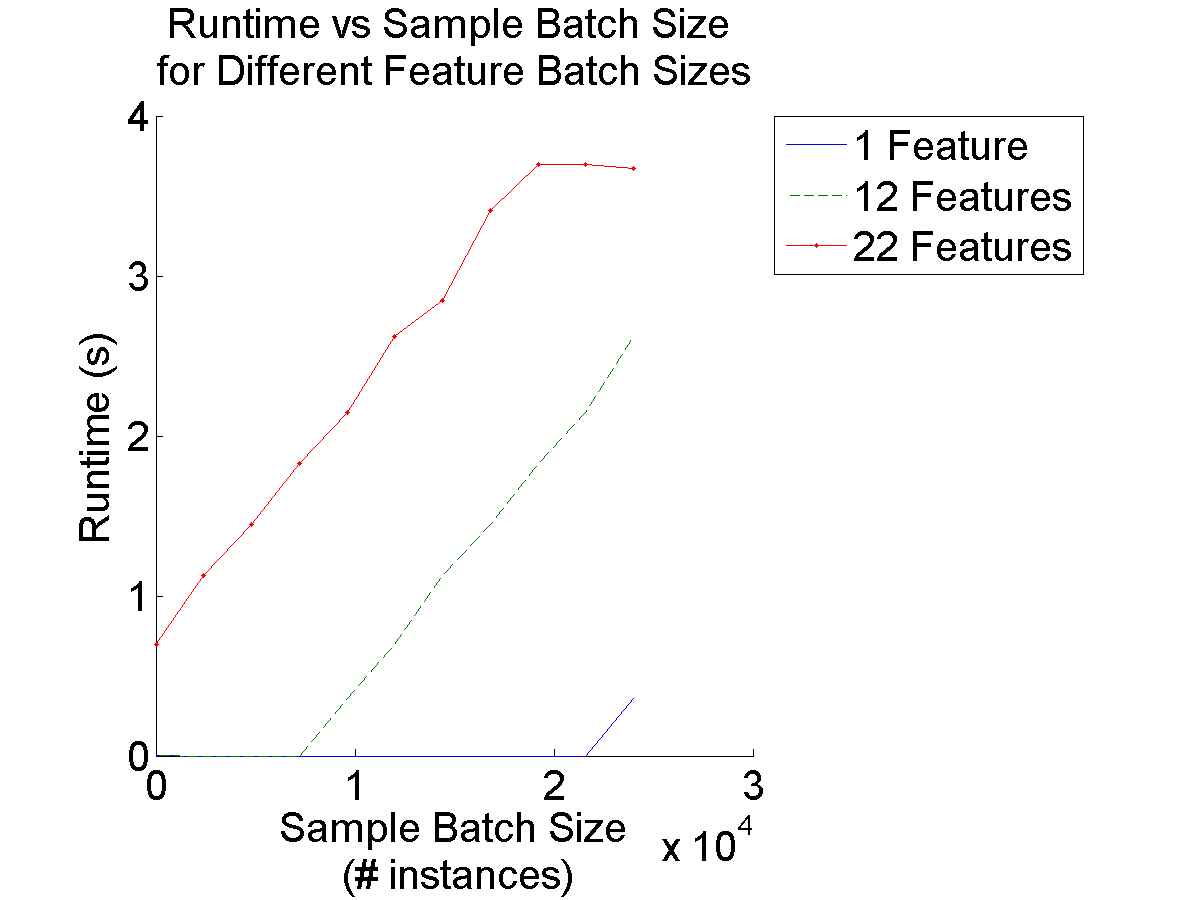
\includegraphics[width = .4\linewidth]{samptimeplot9}
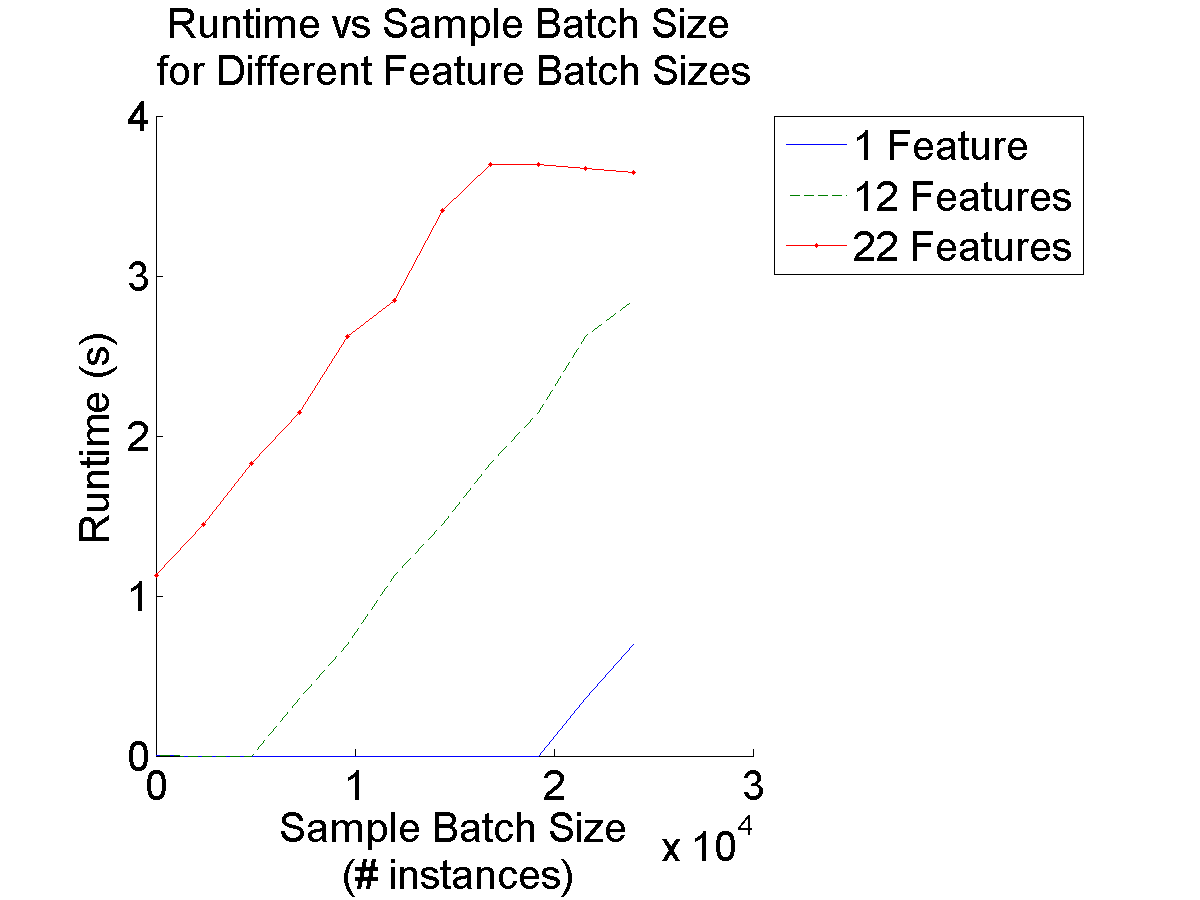
\includegraphics[width = .4\linewidth]{samptimeplot11}
\caption{Runtime versus sample batch size for various feature batch sizes. Upper left is no parallelization, Upper right is parallelization over samples. Bottom left is parallelization over features. Bottom right is parallelization over both.}
\label{fig:time_samp}
\end{figure}
\begin{figure}
\centering
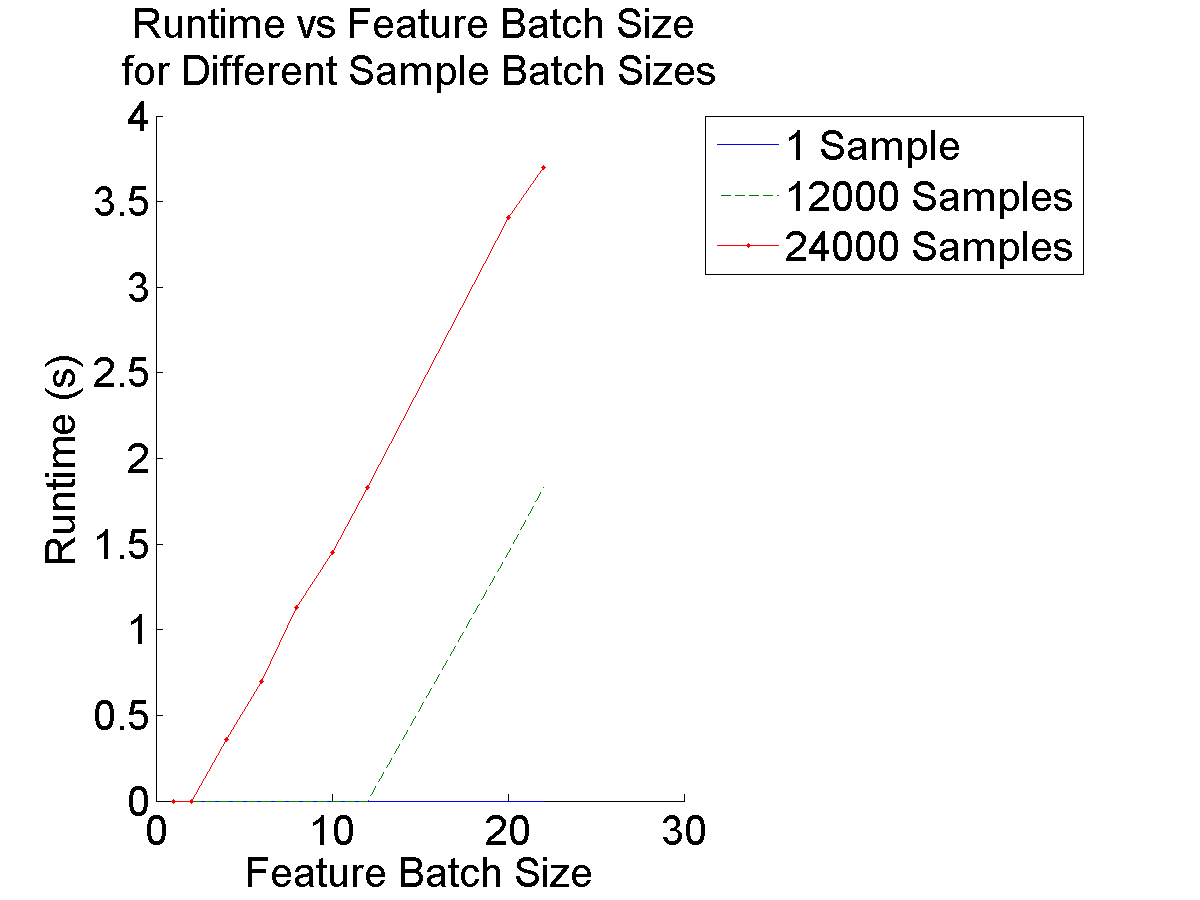
\includegraphics[width = .4\linewidth]{feattimeplot5}
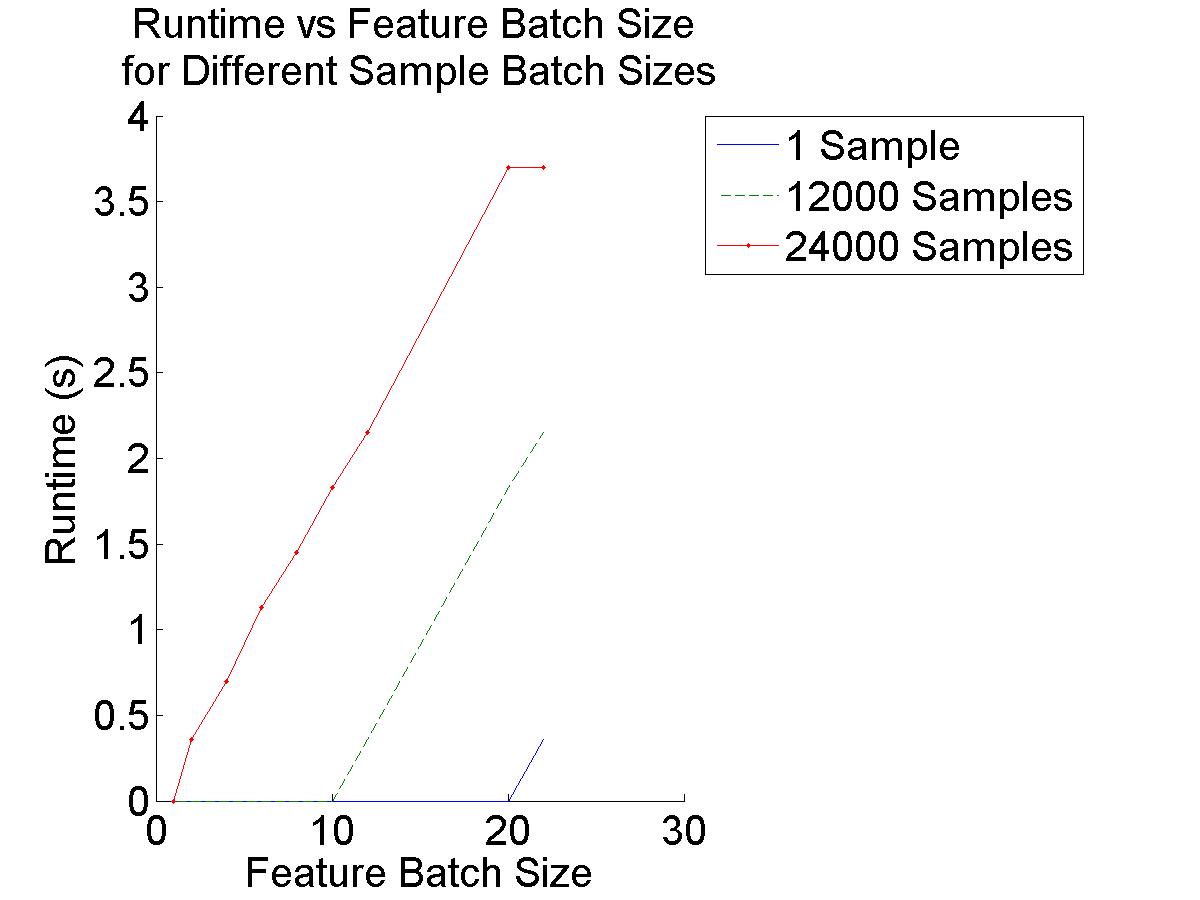
\includegraphics[width = .4\linewidth]{feattimeplot7}
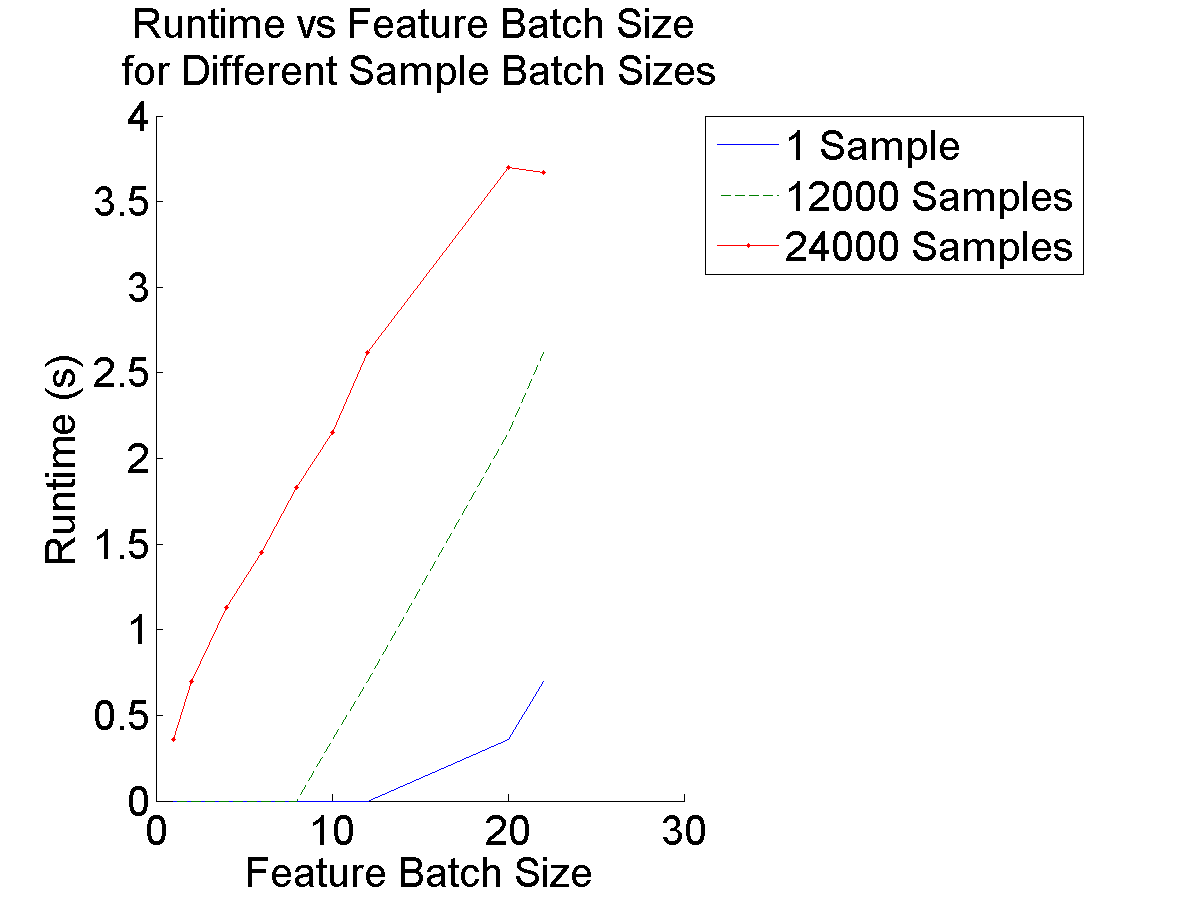
\includegraphics[width = .4\linewidth]{feattimeplot9}
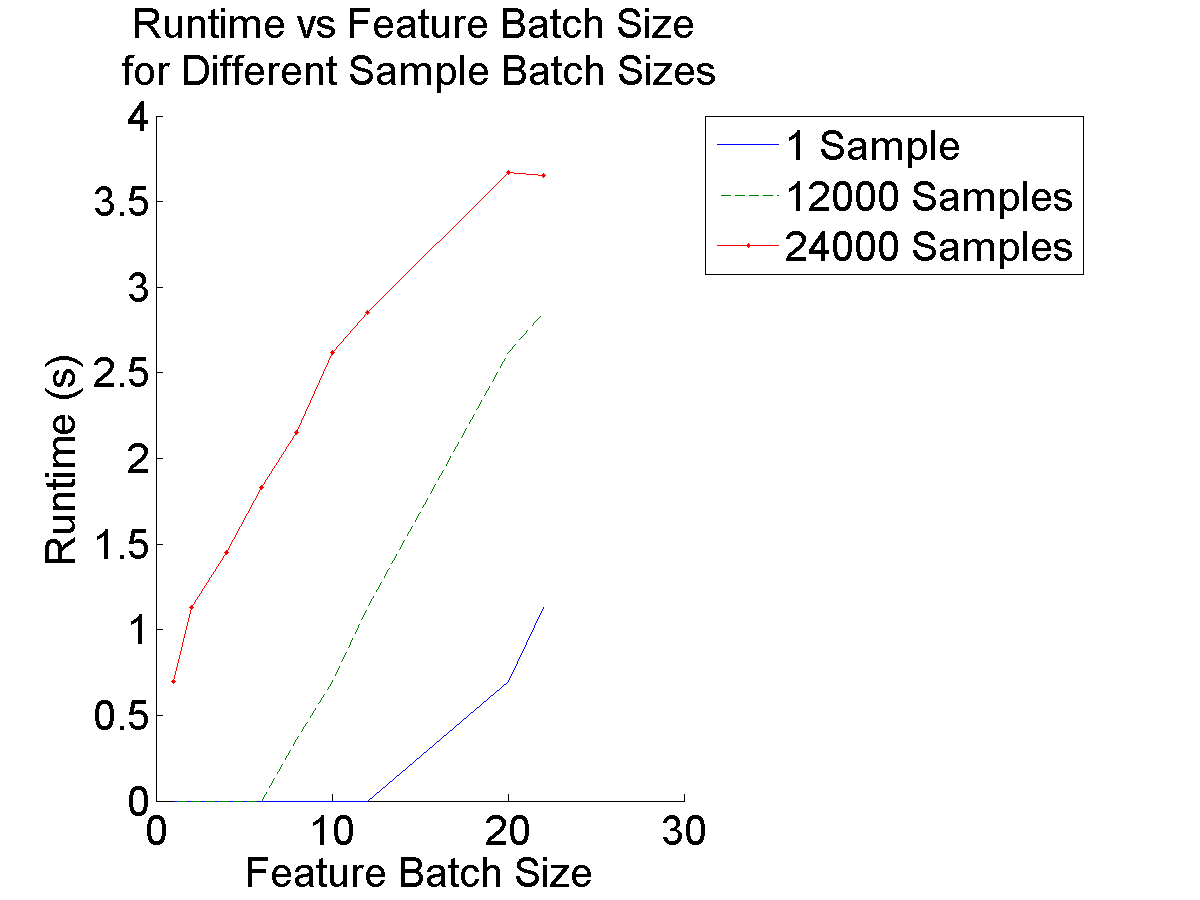
\includegraphics[width = .4\linewidth]{feattimeplot11}
\caption{Runtime versus feature batch size for various sample batch sizes. Upper left is no parallelization, Upper right is parallelization over samples. Bottom left is parallelization over features. Bottom right is parallelization over both.}
\label{fig:time_feat}
\end{figure}
\subsection{Validation Error Analysis}
The effect of parallelization on the error rates is interesting. Parallelizing seems to improve performance for smaller batch sizes, but has a limited effect as batch size increases.  This can be seen when looking at the solid curves in Figures~\ref{fig:err_samp} and \ref{fig:err_feat}.  The largest improvement comes from parallelizing over features, but parallelizing over both loops is still somewhat better.  In general this result is comforting, since most of our updates to the weight vector were not atomic and race conditions were a serious risk, especially for so few total features.
\begin{figure}
\centering
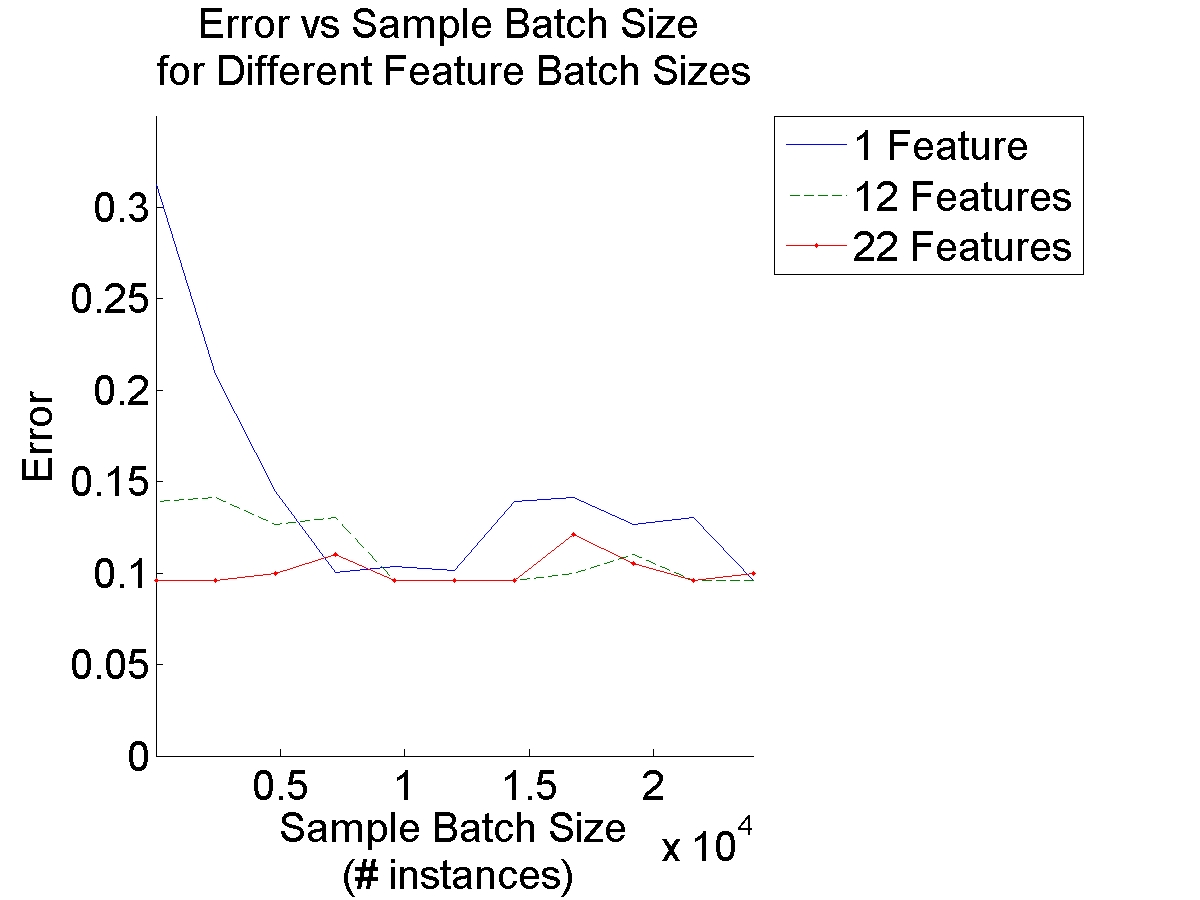
\includegraphics[width = .4\linewidth]{samperrplot6}
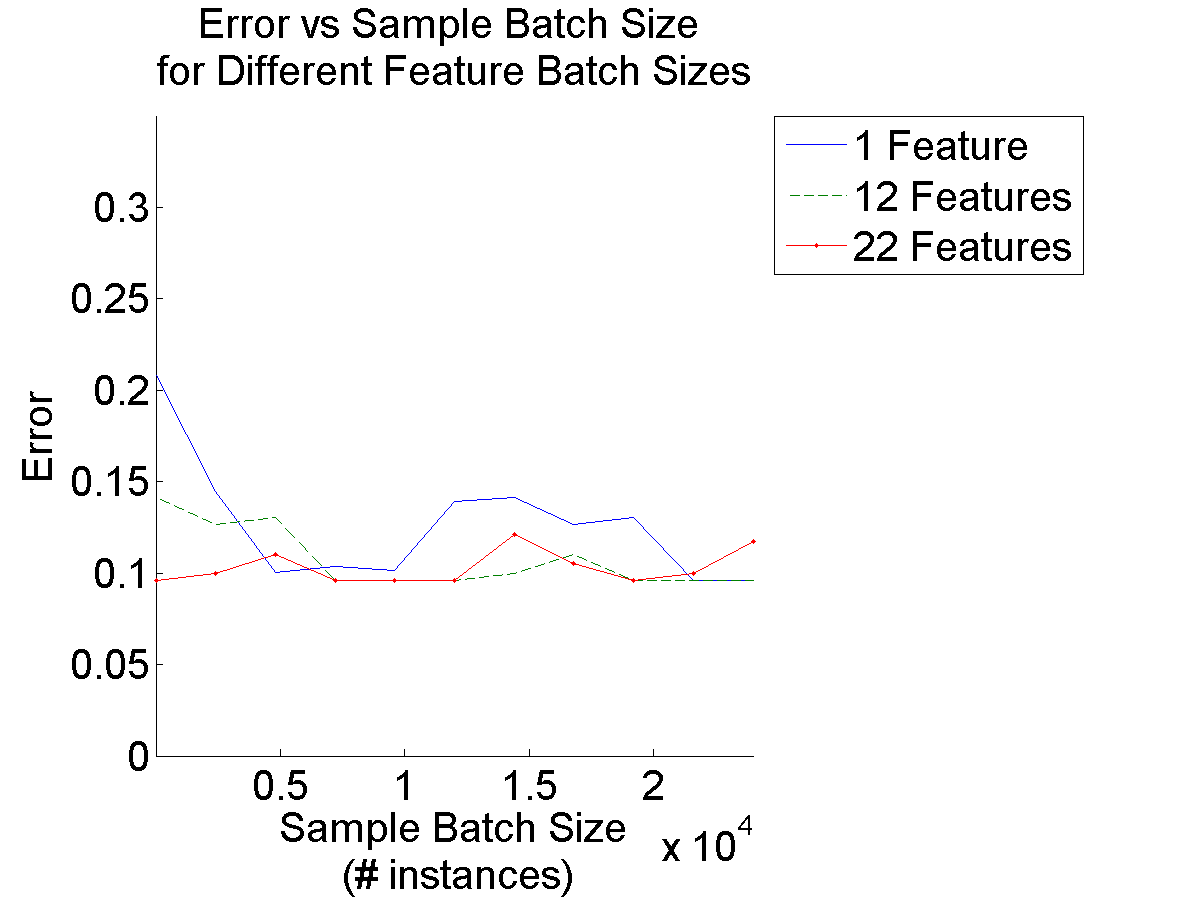
\includegraphics[width = .4\linewidth]{samperrplot8}
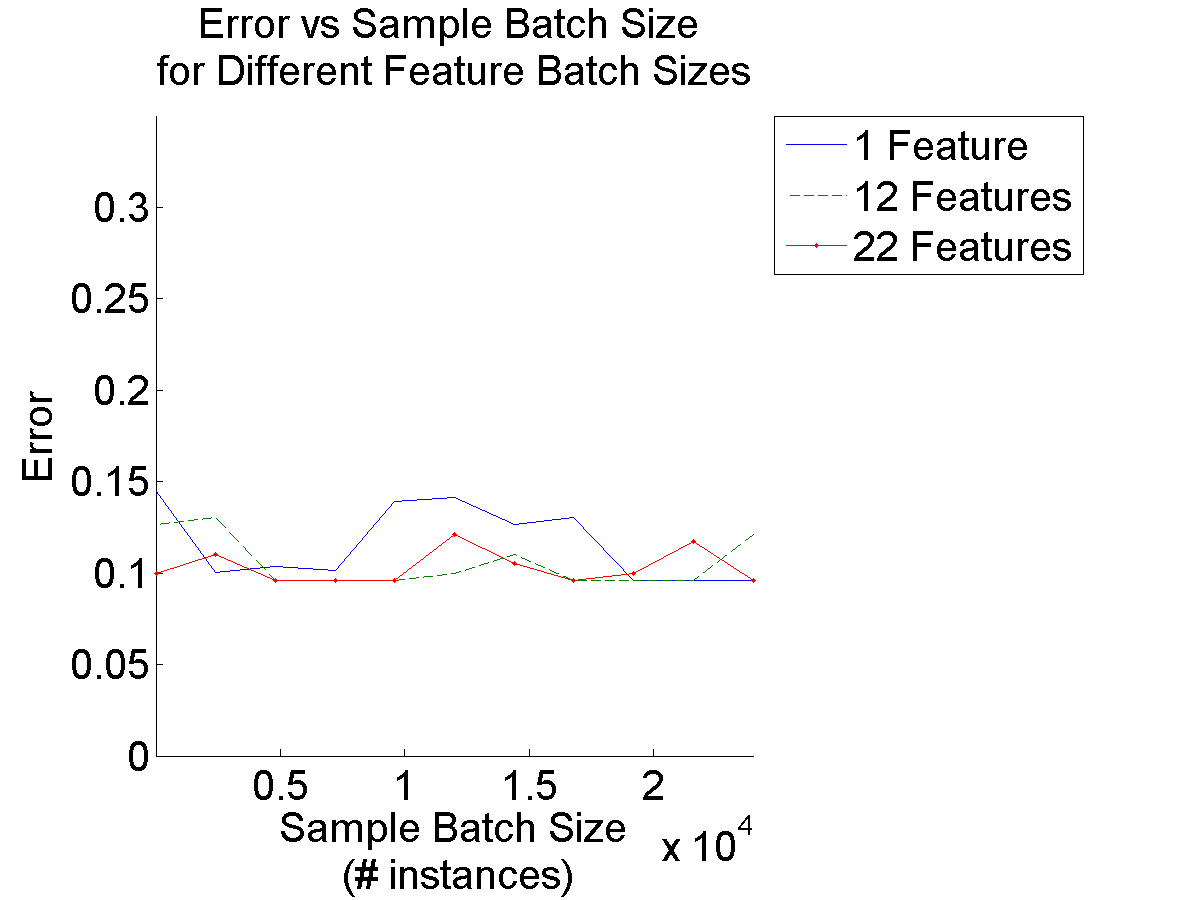
\includegraphics[width = .4\linewidth]{samperrplot10}
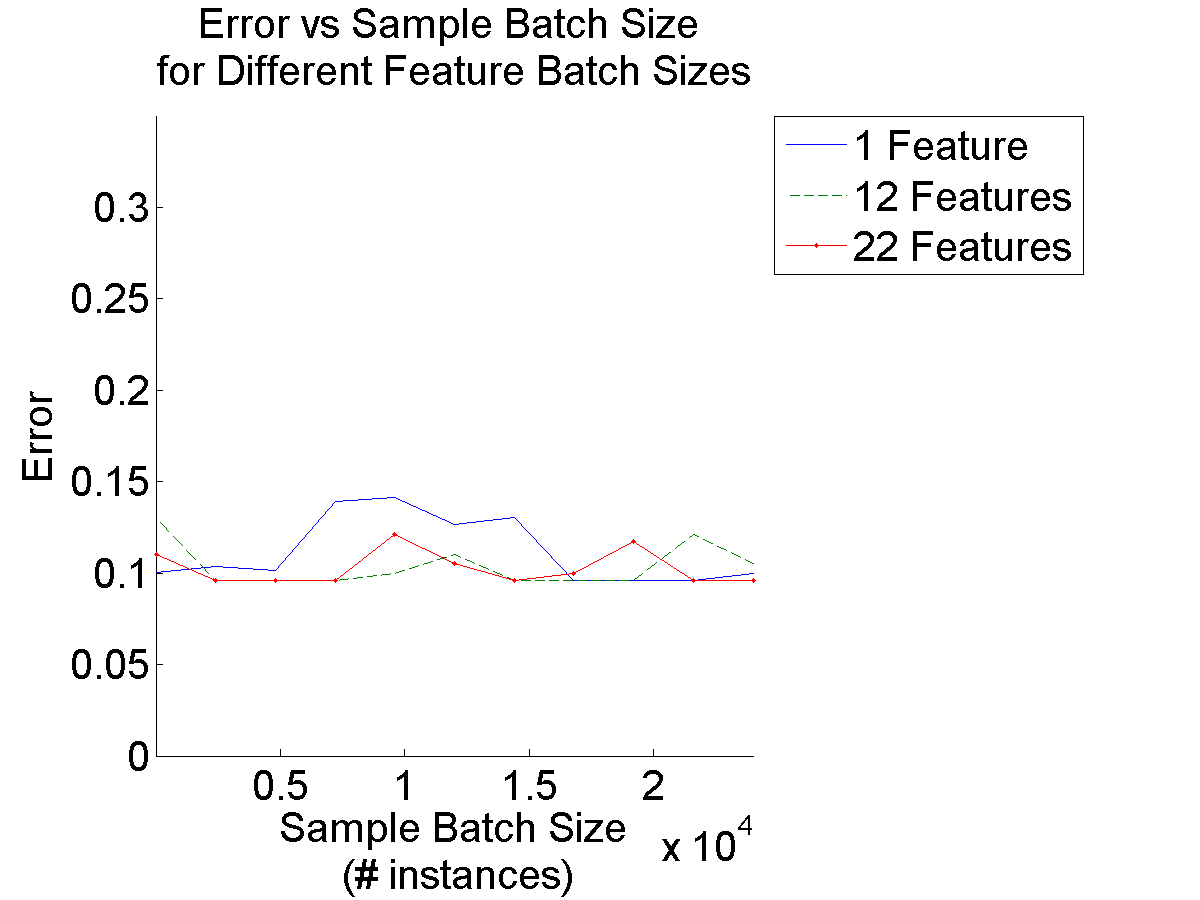
\includegraphics[width = .4\linewidth]{samperrplot12}
\caption{Error versus sample batch size for various feature batch sizes. Upper left is no parallelization, Upper right is parallelization over samples. Bottom left is parallelization over features. Bottom right is parallelization over both.}
\label{fig:err_samp}
\end{figure}
\begin{figure}
\centering
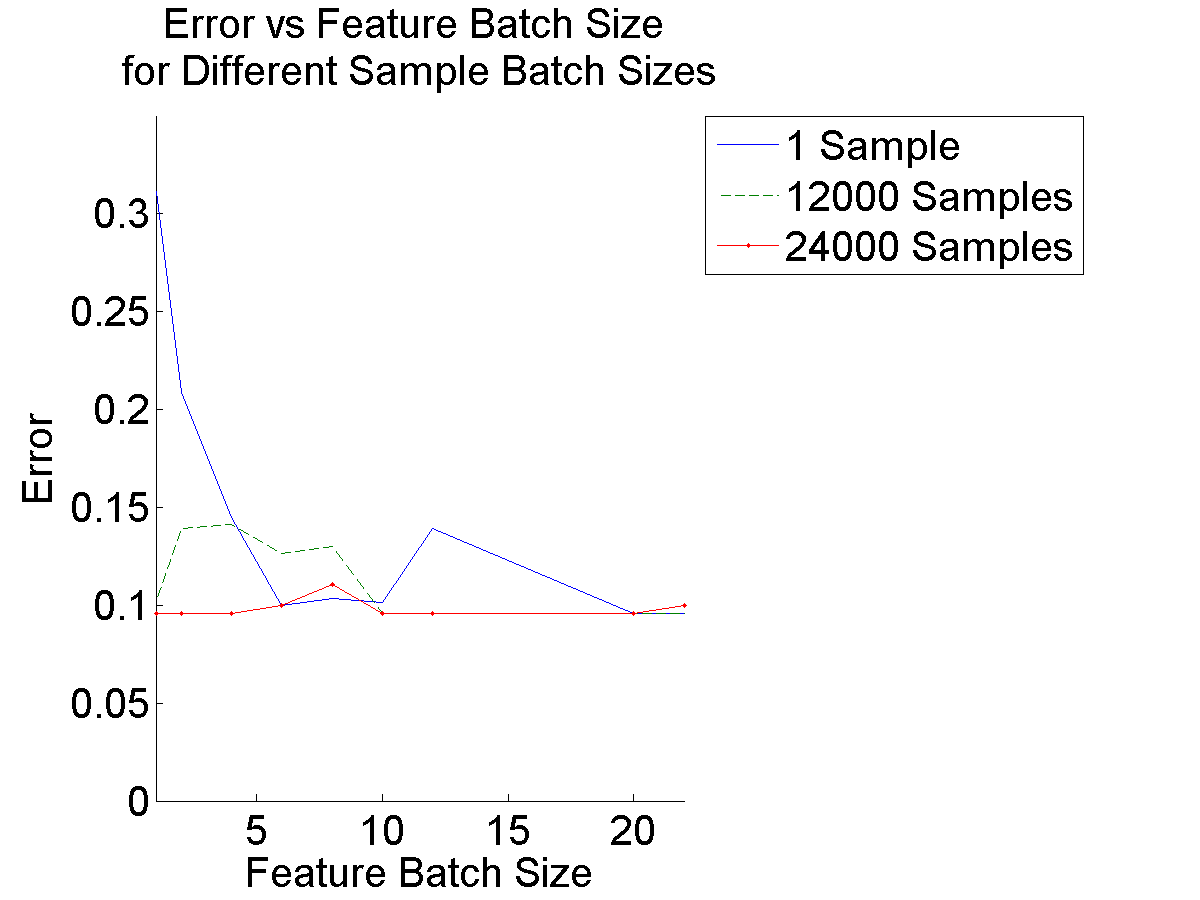
\includegraphics[width = .4\linewidth]{featerrplot6}
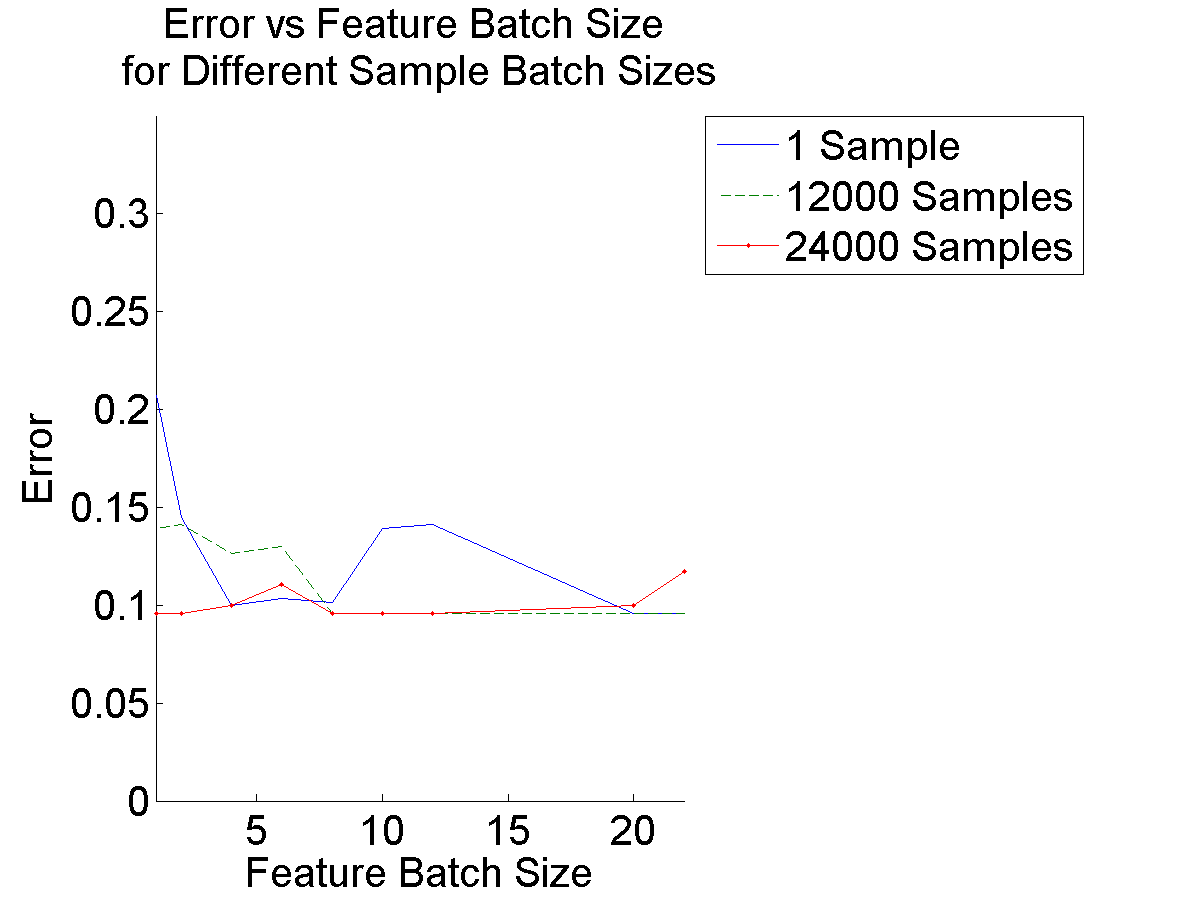
\includegraphics[width = .4\linewidth]{featerrplot8}
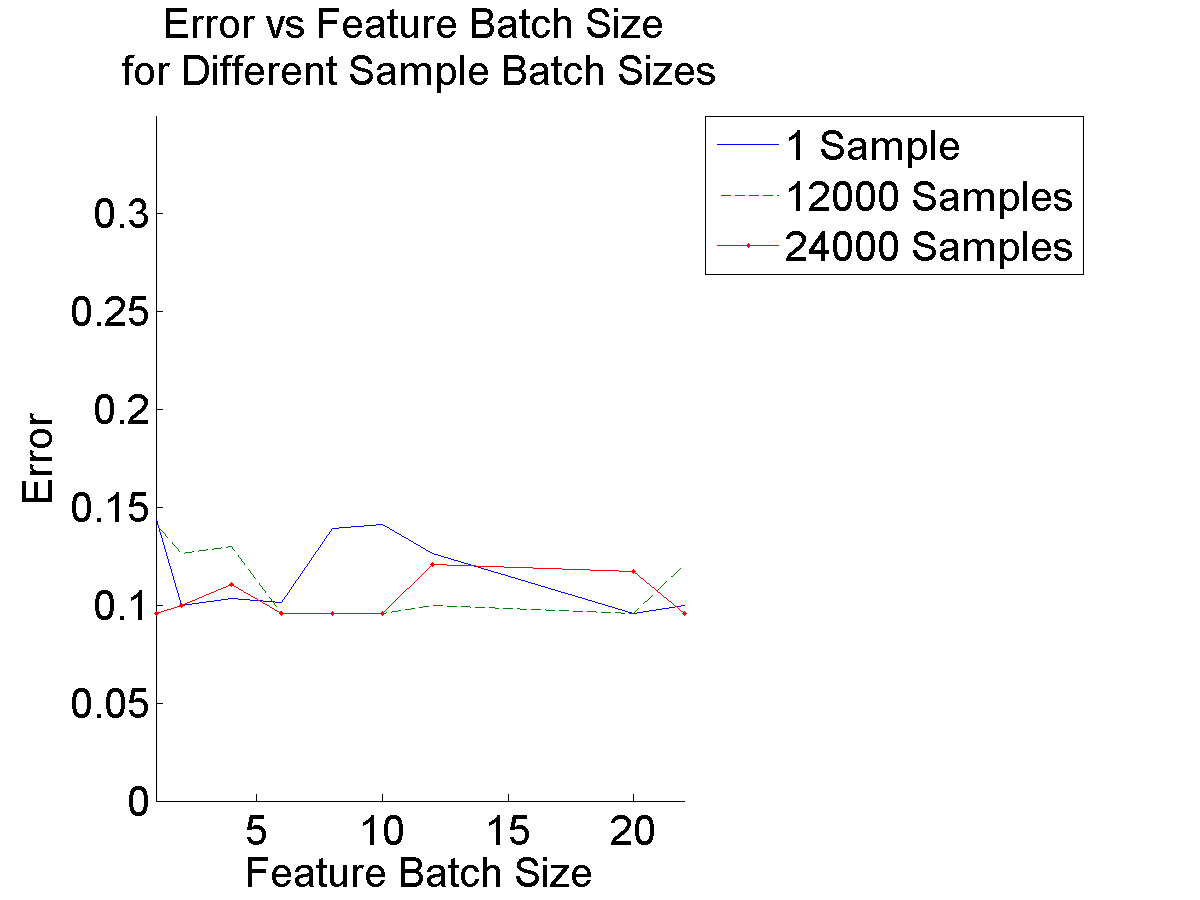
\includegraphics[width = .4\linewidth]{featerrplot10}
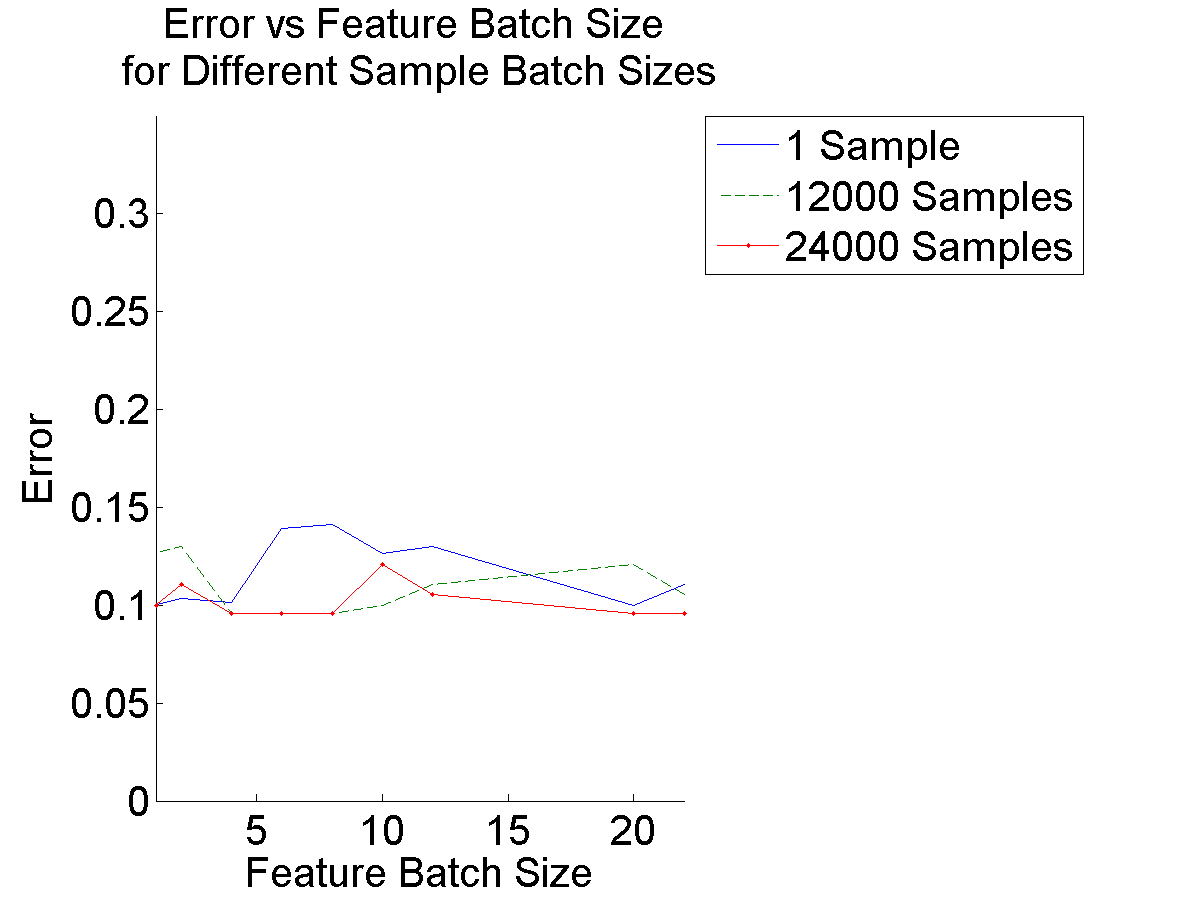
\includegraphics[width = .4\linewidth]{featerrplot12}
\caption{Error versus feature batch size for various sample batch sizes. Upper left is no parallelization, Upper right is parallelization over samples. Bottom left is parallelization over features. Bottom right is parallelization over both.}
\label{fig:err_feat}
\end{figure}
\subsection{Direct Comparison of Parallelization Levels}
To more directly compare the parallelization levels, we have plotted them on the same graphs for the four experimental scenarios in Figure~\ref{fig:parallel}, with lines of best fit. The runtime results (top) are easiest to interpret. It is clear from the intercepts that parallelizing has a startup cost, as previously mentioned. However, the slopes of the lines differ, which double parallelization having the smallest slope. Again, the largest advantage comes from parallelization over features. Examining the error rates is more confusing, due to the high variance in the results.  The error as a function of sample batch size appears much less affected by parallelism, but it seems to make a big difference as a function of feature batch size.
\begin{figure}
\centering
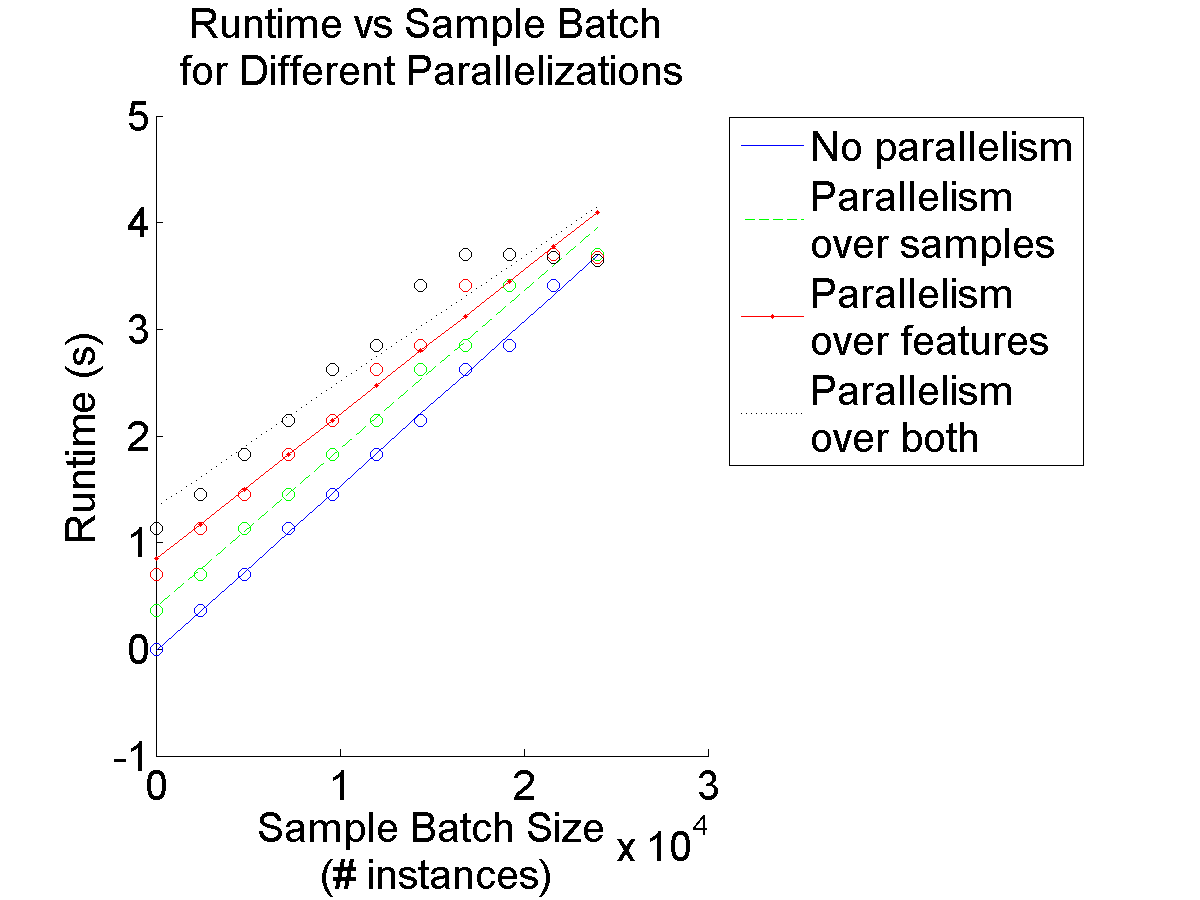
\includegraphics[width = .4\linewidth]{time_samp}
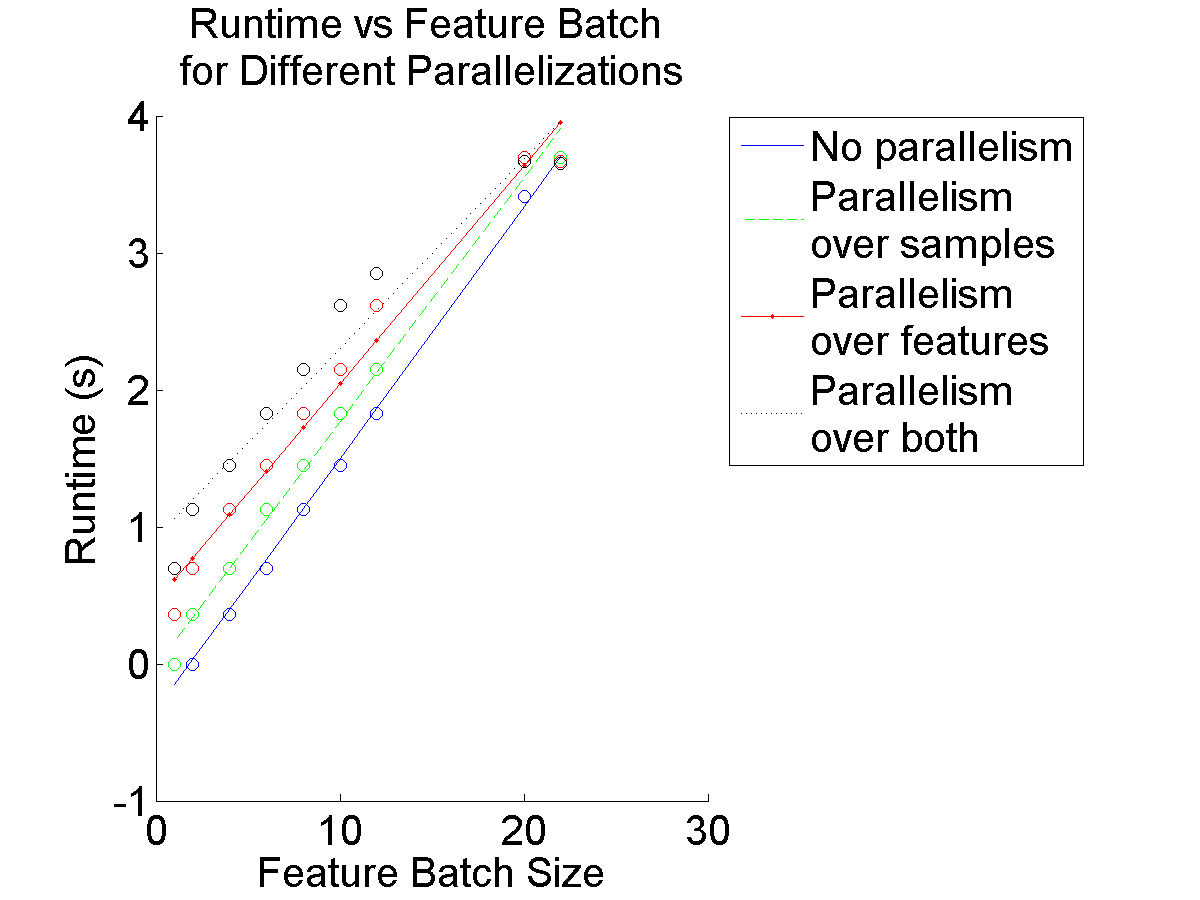
\includegraphics[width = .4\linewidth]{time_feat}
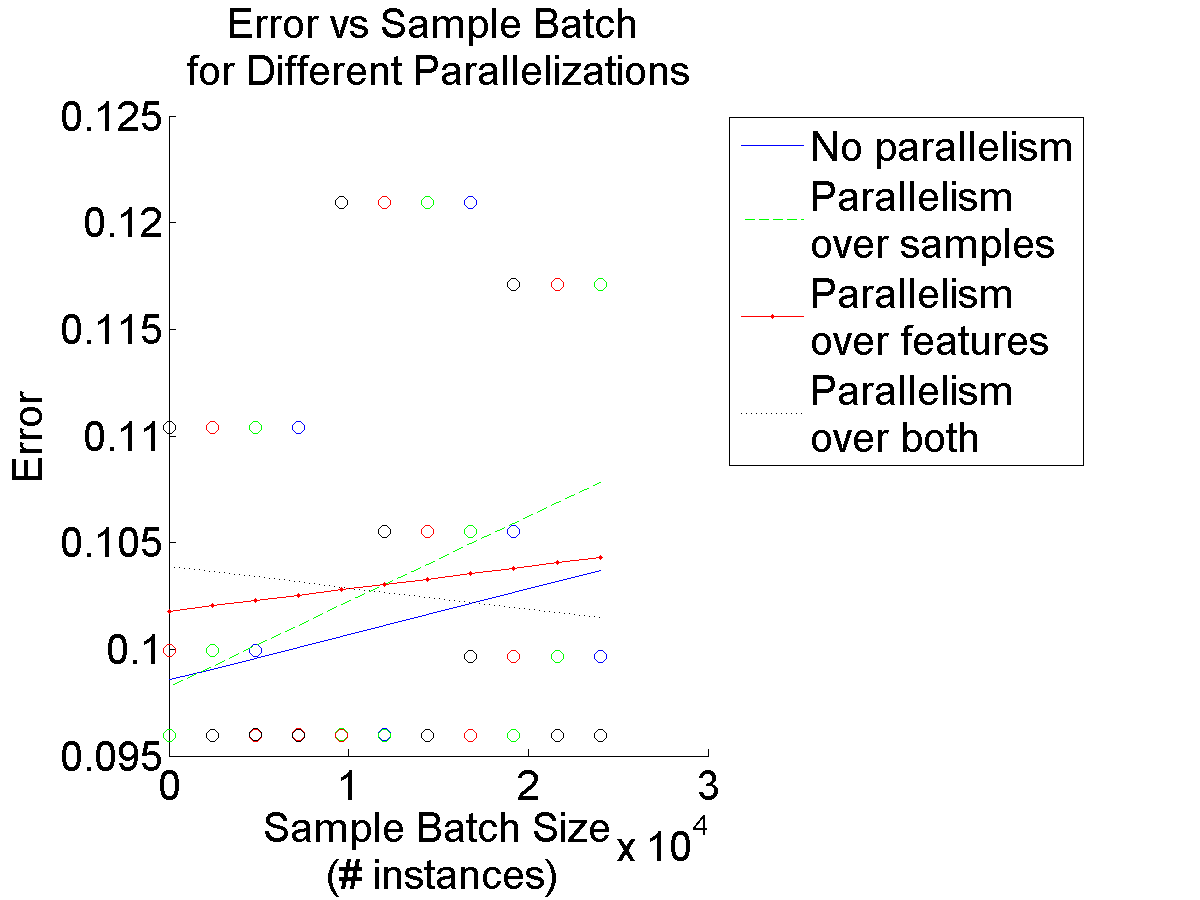
\includegraphics[width = .4\linewidth]{err_samp}
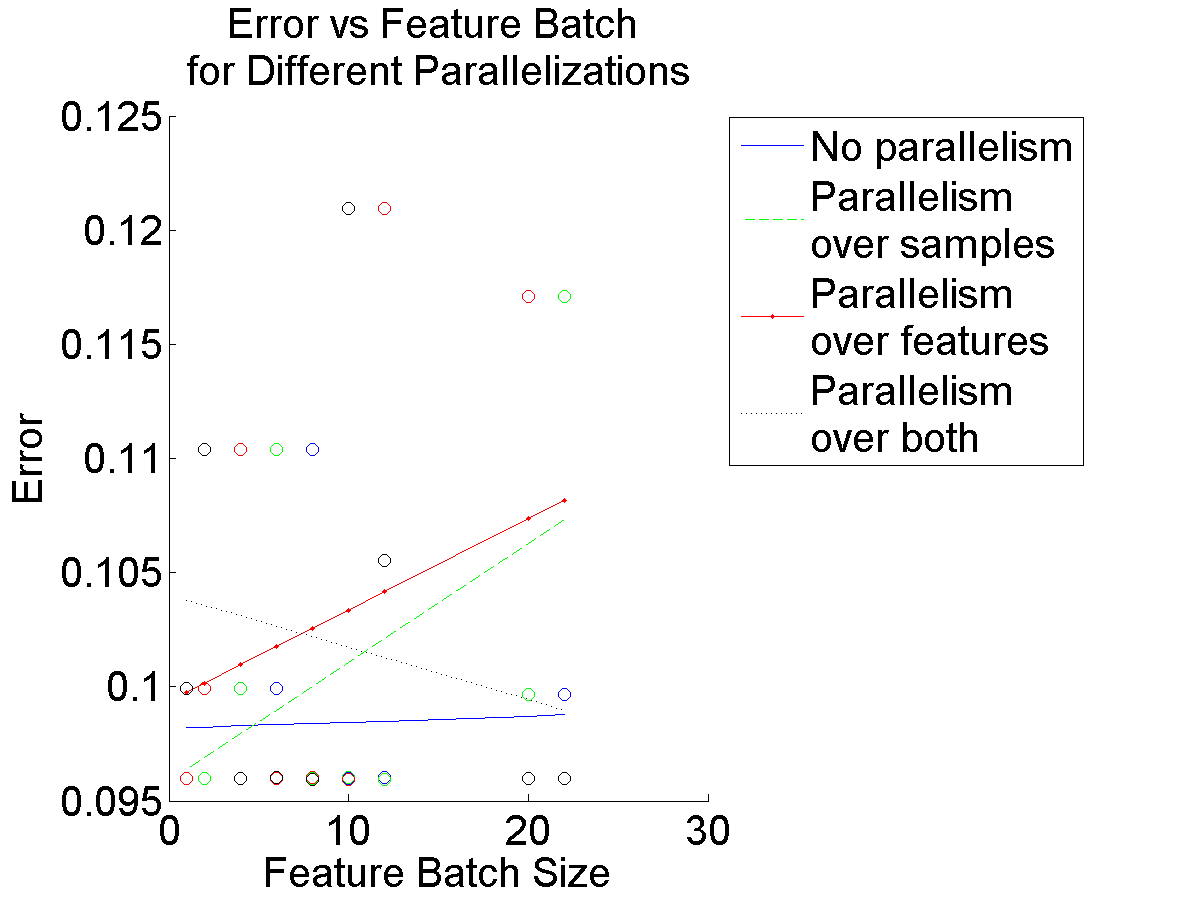
\includegraphics[width = .4\linewidth]{err_feat}
\caption{Direct comparison of parallelization levels. The upper two plots are runtime, and the bottom two are error. Plots on the left vary sample batch sizes and keep feature batch sizes fixed; plots on the right vary feature batch sizes and keep sample batch sizes fixed.}
\label{fig:parallel}
\end{figure}
% Explanation of what figures are what....
% {Runtime, Error} vs. {Feature Batch Size, Sample Batch Size}
%	- Each plot for four levels of parallelization
%	- (there are 16 plots here...might not include them all)
% {Runtime, Error} vs. {Feature Batch Size, Sample Batch Size}
%	- Each plot for both parallelizations: over features and samples
%	- (there are four plots here)

%Figures~\cite{fig:NAME1} through \cite{fig:NAMEn} plot the runtimes and errors as the batch sizes (both features and samples) increase, for various levels of parallelization. As the batch sizes\textemdash both feature batch size and sample batch size\textemdash increase, there is the expected tradeoff between the convergence rate and runtime: when more features or samples are used to update the weights on each iteration, the algorithm converges more quickly, at the expense of more data processing and a longer runtime.

%Of course, the fastest runtime and convergence, for given feature and sample batch sizes, occur when both levels of parallelization are employed. However, Figure~\cite{fig:NAME} indicates that performance improves more significantly when batch updates over features are parallelized than when batch updates over samples are parallelized. This result is likely due to the size of this data set: there are 100 times as many features as samples, so parallelizing over the more computationally-intensive portion of the data set would result in a bigger performance improvement.

\section{Conclusions}
The results demonstrate that while stochastic gradient descent involves many sequential passes through the data, parallelizing it leads to definite runtime improvements without adversely affecting the error convergence properties, in some cases improving the error rate.  As the number of samples and/or features increases, it becomes more beneficial to parallelize across both dimensions.  Even in the case where the number of samples greatly exceeds the number of features, the major benefit arises from parallelizing across features, because it allows multiple features to be updated during an iteration without significant runtime cost.Previous work demonstrated parallelizing either across samples or across features, but we have shown that parallelization is not only possible across both dimensions, but highly useful.

There are some limitations to this project that arose out of time and computing constraints. Firstly, in any experiment involving randomization, it is essential to perform the experiment multiple times and to average the resulting values. This allows estimates to be made with more confidence. Unfortunately, we were unable to do this, and present therefore the results of a single experiment run.  We would also have liked to try the experiments on a data set where the number of features exceeded the number of samples, but we ran out of time.

\bibliographystyle{ieeetr}
\bibliography{refs}

\end{document}
